\documentclass[aspectratio=169]{beamer}

\usepackage[utf8]{inputenc}
\usecolortheme{beaver}
\usepackage{caption}
\usepackage{subcaption}
\usepackage{mathtools}
\usepackage{todonotes}
\usepackage{amsmath}
\usepackage{bm}
\usepackage{listings}
\usepackage{ragged2e}
\usepackage{titlecaps}
\usepackage{fancyvrb}
\usepackage[export]{adjustbox}
\usetikzlibrary{arrows}
\usetikzlibrary{shapes}
\def\ci{\perp\!\!\!\!\!\perp}

\newtheorem{proposition}{Proposition}
\Addlcwords{for a is but and with of in as the etc on to if}

\newcommand{\stackwords}[4]{\begin{tabular}[t]{@{}l@{}l@{}l@{}}#1\\#2\\#3\\#4\end{tabular}}

\setbeamertemplate{section in toc}{\inserttocsectionnumber.~\inserttocsection}
\usetheme{Boadilla}
\makeatletter
\setbeamertemplate{footline}{%
    \leavevmode%
    \hbox{%
        \begin{beamercolorbox}[wd=.3\paperwidth,ht=2.25ex,dp=1ex,center]{author in head/foot}%
            \usebeamerfont{author in head/foot}\insertshortauthor\expandafter\beamer@ifempty\expandafter{\beamer@shortinstitute}{}{~~(\insertshortinstitute)}
        \end{beamercolorbox}%
        \begin{beamercolorbox}[wd=.55\paperwidth,ht=2.25ex,dp=1ex,center]{title in head/foot}%
            \usebeamerfont{title in head/foot}\insertshorttitle
        \end{beamercolorbox}%
        \begin{beamercolorbox}[wd=.15\paperwidth,ht=2.25ex,dp=1ex,right]{date in head/foot}%
            \usebeamerfont{date in head/foot}\insertshortdate{}\hspace*{2em}
            \insertframenumber{} / \inserttotalframenumber\hspace*{2ex} 
        \end{beamercolorbox}}%
        \vskip0pt%
    }
\makeatother

\begin{document}

\title{Testing and Estimation in Causal Models}
\subtitle{Addressing Mixed and Missing Data Challenges}
\author{Ankur Ankan}
\institute[]{Radboud University, The Netherlands}
\date{}

\maketitle

\begin{frame}{Causal Inference}
	\center{Many questions in science are causal.}
	\vspace{1em}
	\only<2>{
	\begin{figure}
		\center
		\begin{subfigure}{0.3 \textwidth}
			\center
			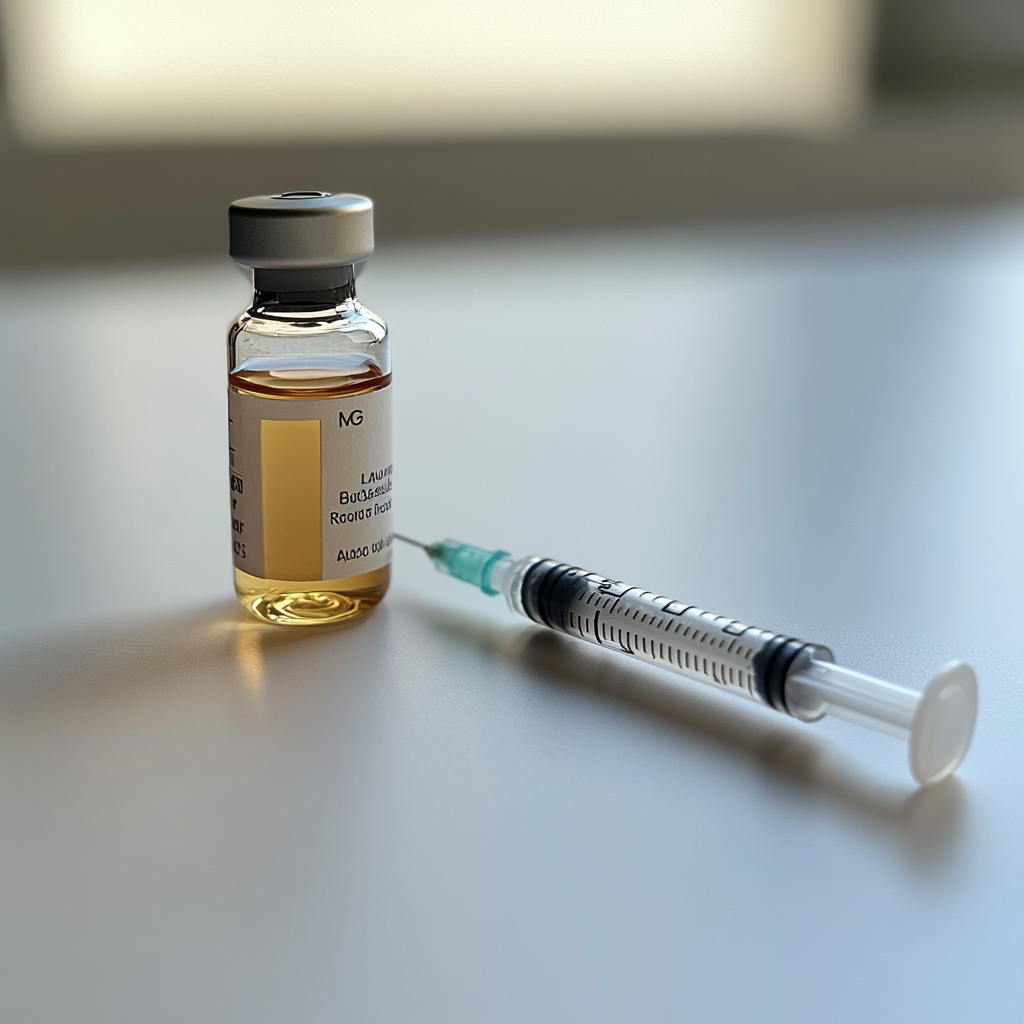
\includegraphics[scale=0.1, valign=m]{imgs/vaccine.png}
		\end{subfigure}
		\qquad\tikz[baseline=-\baselineskip]\draw[ultra thick,->] (-1,0) -- ++ (1,0);\qquad	
		\begin{subfigure}{0.3 \textwidth}
			\center
			
\includegraphics[scale=0.1, valign=m]{imgs/infectious.png}
		\end{subfigure}
	\end{figure}

	\vspace{1em}
	Epidemiology: Does vaccination reduce the spread of infectious disease?
	}
	\only<3>{
	\begin{figure}
		\center
		\begin{subfigure}{0.35 \textwidth}
			\center
			
\includegraphics[scale=0.1, valign=m]{imgs/video_game.png}
		\end{subfigure}
		\qquad\tikz[baseline=-\baselineskip]\draw[ultra thick,->] (0,0) -- ++ (1,0);\qquad	
		\begin{subfigure}{0.35 \textwidth}
			\center
			
\includegraphics[scale=0.1, valign=m]{imgs/fight.png}
		\end{subfigure}
	\end{figure}
	\vspace{1em}
	Social Science: Does exposure to violent video games increase aggressive behavior in children?
	}
	\only<4>{
	\begin{figure}
		\center
		\begin{subfigure}{0.35 \textwidth}
			\center
			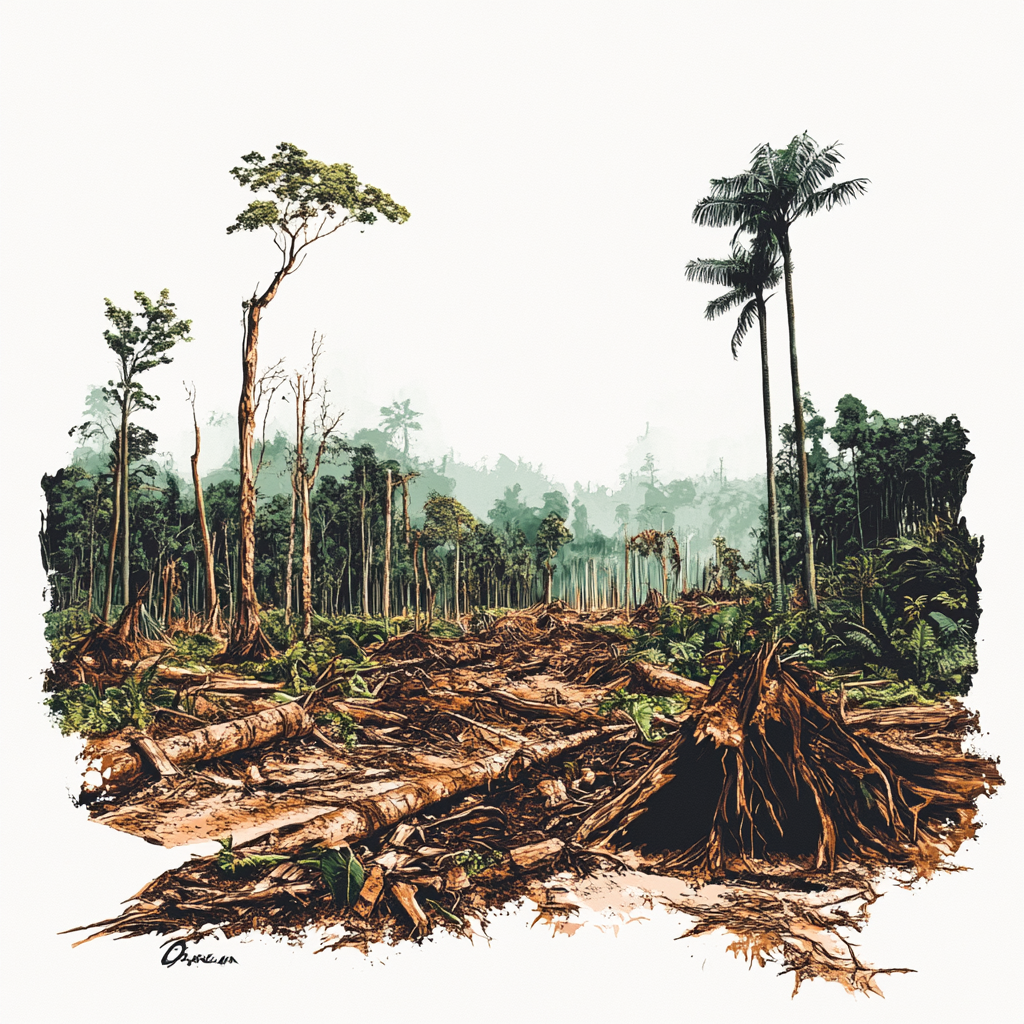
\includegraphics[scale=0.1, valign=m]{imgs/deforestation.png}
		\end{subfigure}
		\qquad\tikz[baseline=-\baselineskip]\draw[ultra thick,->] (0,0) -- ++ (1,0);\qquad	
		\begin{subfigure}{0.35 \textwidth}
			\center
			
\includegraphics[scale=0.1, valign=m]{imgs/climate_change.png}
		\end{subfigure}
	\end{figure}
	\vspace{1em}
	Environmental Science: Does deforestation contribute to climate change?
	}
\end{frame}

\begin{frame}{Causal Inference}
	\begin{tabular}{cccc}
		Understand how an \textbf{intervention} on an & \textbf{exposure} & influences an & \textbf{outcome}. \\
							      & vaccination & & infection spread \\
							      & video games & & aggressive behavior \\
							      & deforestation & & climate change \\
	\end{tabular}
	\vspace{2em}

	\only<2>{
		\begin{itemize}
		\item \textbf{Understanding Causal Relationships: }
			\begin{itemize}
				\item Is there a causal relationship between the exposure and the outcome?
				\item What kind of relationship? Direct, indirect, and so on.
			\end{itemize}
		\item \textbf{Quantifying Causal Relationships: }
			\begin{itemize}
				\item Measure the magnitude of the intervention's impact.
				\item For example, by how much would vaccination reduce spread of infection?
			\end{itemize}
		\end{itemize}
	}
\end{frame}

\begin{frame}{Randomized Controlled Trials}
	\center{Best way to answer these causal questions is using \textbf{Randomized Controlled Trials}.}
	\vspace{1em}
	\begin{figure}
		\center
		\includegraphics[page=8]{figures.pdf}
	\end{figure}

	\vspace{0.5em}
	\only<2>{
		\begin{itemize}
			\item Understanding Causal Relationships: A significant difference in infection spread implies a causal relationship.
			\item Quantifying Causal Relationships: The difference in the infection spread.
		\end{itemize}
	}
\end{frame}

\begin{frame}{Randomized Controlled Trials}
	\center{However, randomized controlled trials are \textbf{not always feasible.}}
	
	\vspace{2em}

	\begin{itemize}[<+->]
		\item \textbf{Unethical: } To study the effect of smoking on lung cancer, we cannot ask non-smokers to start smoking.
		\item \textbf{Difficult to control exposures:} To study the effects of deforestation on climate, we cannot create clones of Earth.
		\item \textbf{Cost:} Studying the effect of education on income would require decades of tracking individuals.
	\end{itemize}

	\vspace{2em}

\only<4>{
\center{Can we answer these questions using non-experimental data?}
}
\end{frame}

\begin{frame}{Causal Graphs}
	\center{Yes, but requires understanding the causal mechanism.}
	\vspace{0.5em}
	\begin{figure}
		\begin{overprint}
			\onslide<1> \center \includegraphics[page=1]{figures.pdf}
			\onslide<2> \center \includegraphics[page=2]{figures.pdf}
			\onslide<3> \center \includegraphics[page=3]{figures.pdf}
			\onslide<4> \center \includegraphics[page=4]{figures.pdf}
			\onslide<5> \center \includegraphics[page=4]{figures.pdf}
		\end{overprint}
	\end{figure}

\only<5>{
	\begin{itemize}
		\item Understanding causal relationships $ \implies $ Constructing the causal graph.
		\item Quantifying causal relationships $ \implies $ Estimating the edge strengths.
	\end{itemize}
}
\end{frame}

% \begin{frame}{Mixed and Missing Data}
% 	\center{I have focused on improving these methods for mixed and missing data.}
% 
% 	\vspace{2em}
% 
% 	\begin{itemize}
% 		\item \textbf{Mixed Data:}
% 			\begin{enumerate}
% 				\item Numerical:
% 				\item Categorical:
% 				\item Ordinal:
% 			\end{enumerate}
% 
% 		\item \textbf{Missing Data:} Not all variables can be measured. For example climate change.
% 	\end{itemize}
% \end{frame}

\begin{frame}{Constructing Causal Graphs}
	\center{How to construct causal graphs?}
	
	\vspace{2em}
	
	\begin{itemize}
		\item Usually constructed manually based on domain knowledge.
		\item Important to test whether our causal graph is correct.
	\end{itemize}
	
	\vspace{1em}
	
	\begin{figure}
		\center
		\includegraphics[page=5]{figures.pdf}
	\end{figure}
	
\end{frame}

\begin{frame}{Testing Causal Graphs}
	\begin{itemize}
		\item Selecting the appropriate conditional independence test depends on a
	lot of factors.
		\item One of the main factors is type of variables:
			\begin{itemize}
				\item Numerical: Area of deforestation.
				\item Categorical: 
				\item Ordinal:
			\end{itemize}
	\end{itemize}

	\vspace{2em}
		
	\center{We wrote a comprehensive guide for selecting appropriate tests for their data.}
\end{frame}

\begin{frame}{Constructing Causal Graphs}
	\begin{figure}
		\center
		\includegraphics[page=6]{figures.pdf}
	\end{figure}

	\begin{itemize}
		\item Both model testing and automatically constructing graphs rely on the accuracy of tests.
		\item Incorrect tests $ \implies $ Incorrect edges.
	\end{itemize}

	\vspace{0.5em}
	
	\center{We proposed a new conditional independence test.}
\end{frame}

\begin{frame}{Causal Effect Estimation}
	\begin{columns}
		\begin{column}{0.65 \textwidth}
			\begin{itemize}
				\item Easy to estimate if we can measure the variables.
				\item But not always possible to measure variables.
				\item Example, climate change cannot be measured directly.
				\item But other variables can be used to measure them. For climate change we can use:
					\begin{itemize}
						\item Global average temperature
						\item Sea level rise
						\item Atmospheric CO2 concentration
					\end{itemize}
			\end{itemize}
		\end{column}
		\begin{column}{0.38 \textwidth}	
			\begin{figure}
				\center
				\includegraphics[page=7]{figures.pdf}
			\end{figure}
		\end{column}
	\end{columns}

	\vspace{2em}
	
	\center{We developed a new method to be able to estimate effects between such variables that can not be measured directly.}
\end{frame}

\begin{frame}{Future Research}
	\begin{itemize}
		\item Plan to further improve the conditional independence test that we proposed.
		\item Combine conditional independence testing and estimation methods to come up with an interpretable metric for mixed data.
	\end{itemize}
\end{frame}

\end{document}
